\section{Introduction}

written at the end of project
IN GENERAL
\begin{enumerate}
\item goal of project
\item importance of goal
\item how will goal be achieved
\item overview of main sections in report
\end{enumerate}

In Belgium one man in three and one woman in four faces cancer before his or
her 75th birthday \cite{kanker}. In 2010 62 017 new cases of cancer were
diagnosed in Belgium \cite{kankerliga}. The World Health Organisation estimates
the worldwide death toll from lung cancer will be 10 000 000 by 2030, which
makes it one of the deadliest cancers \cite{gu, zheng}.
However, an early detection can increase the survival rate up to 70-80\%
\cite{swensen}. Furthermore, research has shown that the detection of lung
cancer in an early stage broadens the amount of treatment options and increases
the amount of invasive surgery\cite{greenlee}.


Due to recent developments in
computed tomography (CT) technology it is now possible to obtain near isotropic,
submillimeter resolution images of the complete chest in a single breath hold.
This high resolution has the advantage that it enables visualisation of small
and low-contrast nodules that could hardly be screened in conventional
programs. The downside is that enormous amounts of data are generated
which increases the work load of radiologists, especially since low-dose CT
scans are more and more implemented in routine screenings. Still, this is no
idle measure. Long nodules are very commonly detected on CT scans. Research
shows that up to 51\% of smokers aged 50 years or older have pulmonary lung
nodules on CT scans \cite{mahon}. Therefore, the United States Preventive
Services Task Force for example stated that it ``recommends annual screening for
lung cancer with low-dose computed tomography (LDCT) in adults aged 55 to 80
years who have a 30 pack-year smoking history and currently smoke or have quit
within the past 15 years'' \cite{ups}.
Therefore, the detection of pulmonary nodules from volumetric computed
tomography (CT) scans if one of the most studied CAD applications
\cite{sluimer}.


Currently, expert radiologists perform the investigation of the
CT scans. They use the shape, the texture, the location and the growth rate of
the volume of the nodule as clinical parameter to determine the malignancy of
the nodules and to decide on the diagnosis of lung cancer. A jagged shape
nodule is more likely to be lung cancer than a smooth one. A fatty, bony,
watery nodule or a mixture of these different contents is less likely to
indicate lung cancer than a nodule that is attached to a vessel. A nodule
attached to the lung wall is typically diagnosed as benign if the
volume-doubling periode is longer than 400 days \cite{wu}. Nevertheless, the
examination of these scans is a time-consuming task and is not free from errors.
Although small nodules are in principle detectable in CT scans, a non-negligible
fraction may be overlooked if they are situated in a maze of vessels of similar
size \cite{ozekes}. An example of a nodule hidden in a maze of vessels is shown
in \ref{nodmaze}.
\begin{figure}[htp]
\begin{center}
  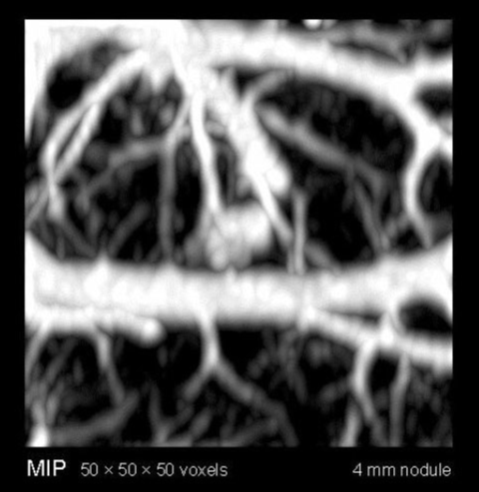
\includegraphics[width= 30 mm]{img/noduleMaze.png}
  \caption{Nodule in maze of vessels of similar size \cite{noduleMaze}.}
  \label{nodmaze}
\end{center}
\end{figure}
Another problem that arises is the intra- and interreader variability
amongst radiologists in pulmonary lung detection \cite{armato} \cite{hens}. Therefore,
there is a need for a computer-aided detection (CAD) system that can assist the
radiologist in the detection of pulmonary nodules.

VERDER
contributions of the paper: explore the use of ensemble classifier RF in nodule detection (not first nodule
segmentation)
fast + accurate


mission definition:

The goal of this project is to develop a fully automated algorithm for the
detection of lung nodules, based on assumptions about the shape and appearance of their
features. An algorithm based on machine learning techniques will be used to
tackle this goal. One of the challenges is the selection of the features. The
fact that some nodules are embedded in surrounding tissue (e.g.
lung wall, blood vessel, etc.) presents another important challenge.



